\documentclass[10pt,a4paper]{article}
\usepackage[margin=2cm]{geometry}
\usepackage[T1]{fontenc}
\usepackage{lmodern}
\usepackage{amsmath,amssymb}
\usepackage{booktabs,tabularx,array}
\usepackage{xcolor}
\usepackage{enumitem}
\usepackage{tikz}
\usetikzlibrary{positioning,arrows.meta,calc}
\usepackage{graphicx}
\usepackage[colorlinks=true,linkcolor=blue!50!black,urlcolor=blue!50!black]{hyperref}
\setlist{itemsep=1pt,topsep=2pt}
\setlength{\parskip}{3pt}
\setlength{\parindent}{0pt}

\definecolor{ex}{HTML}{DCEBFB}
\definecolor{lp}{HTML}{FCE3D5}
\definecolor{dat}{HTML}{E2F2DF}
\definecolor{ink}{HTML}{1F2328}
\definecolor{accent}{HTML}{2A78D6}
\definecolor{warn}{HTML}{C2410C}
\definecolor{essA}{HTML}{C2410C}
\definecolor{essB}{HTML}{0B7285}

\tikzset{
  box/.style={draw=ink!70, rounded corners=2pt, align=center, font=\small, inner sep=4pt, minimum height=7mm},
  lpbox/.style={box, fill=lp},
  datbox/.style={box, fill=dat},
  arr/.style={-{Stealth[length=2.2mm]}, thick, ink!75},
  darr/.style={-{Stealth[length=2.2mm]}, thick, dashed, ink!55},
  lab/.style={font=\scriptsize\itshape, text=ink!70, fill=white, inner sep=1pt},
}

\newcommand{\code}[1]{\texttt{#1}}
\newcommand{\lamstar}{\lambda^{\star}}
\newcommand{\lamhat}{\hat\lambda}
\newcommand{\what}{\hat w}

\title{\textbf{Stage 1 structure}\\[2pt]
\large Two batteries on one bus, with an error in each owner's terminal value}
\author{Companion to \code{docs/model\_structure.pdf}\\\small Figures and numbers: \code{scripts/make\_stage1\_figures.py}}
\date{28 October 2026}

\begin{document}
\maketitle
\vspace{-6mm}

\begin{center}
\fbox{\begin{minipage}{0.93\textwidth}\small
\textbf{What stage 1 adds.} Stage 0 had one battery and one error, the price forecast $\lamhat$. Stage 1
keeps the same system but splits the battery into \textbf{two batteries, A and B}, owned separately, and adds
a \textbf{second error}: each owner's estimate $\what_e$ of its own end-of-horizon value $w_e$. Baldick's
design is again the benchmark; the question is how much welfare the current design loses when two owners
build their bids independently, each from its own price forecast and its own estimate of what stored energy
is worth at the end of the day.
\end{minipage}}
\end{center}

\tableofcontents

% =====================================================================
\section{Big picture}
% =====================================================================
The comparison is the one of stage 0: a benchmark welfare $SW^\star$ from Baldick's design, solved once,
against the realised welfare $SW_{\text{real}}$ of the current design. What changes is the lower path: two
owners now build their bids separately, each with two errors, and the two bids meet in one market.

\begin{center}
\resizebox{\textwidth}{!}{%
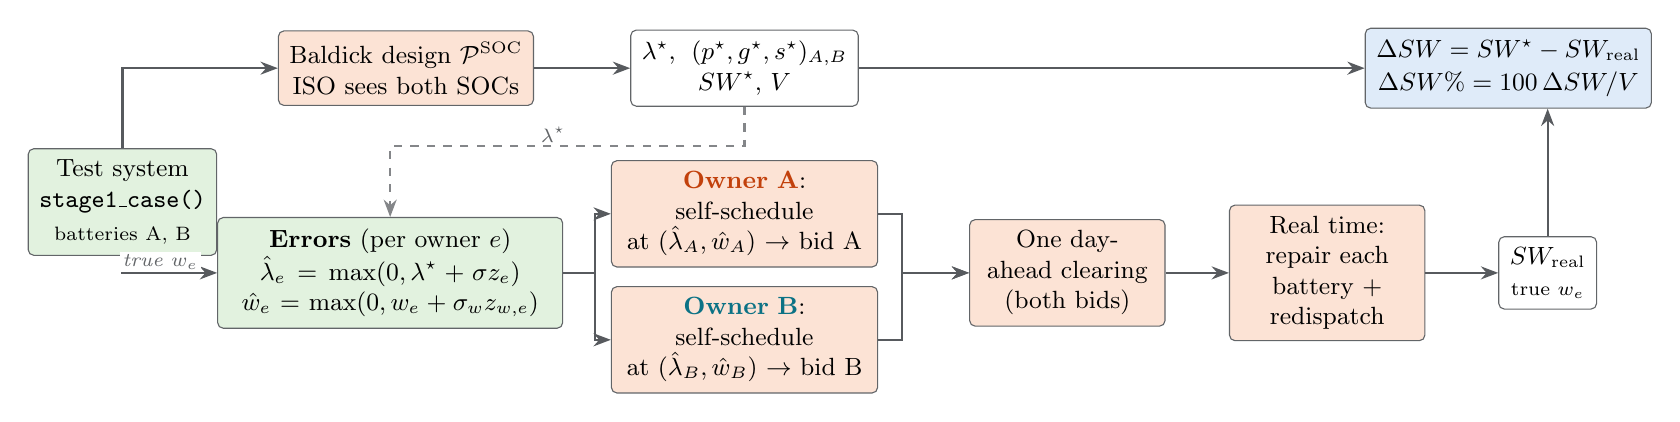
\begin{tikzpicture}
  \node[datbox] (case) at (0,0) {Test system\\\code{stage1\_case()}\\[1pt]\scriptsize batteries A, B};
  \node[lpbox] (soc) at (3.6,1.7) {Baldick design $\mathcal P^{\text{SOC}}$\\ISO sees both SOCs};
  \node[box] (star) at (7.9,1.7) {$\lamstar$,\; $(p^\star,g^\star,s^\star)_{A,B}$\\$SW^\star$, $V$};
  \node[datbox, text width=4.1cm] (err) at (3.4,-0.9) {\textbf{Errors} (per owner $e$)\\[1pt]
        $\lamhat_e=\max(0,\lamstar+\sigma z_e)$\\$\what_e=\max(0,w_e+\sigma_w z_{w,e})$};
  \node[lpbox, text width=3.1cm] (oA) at (7.9,-0.15) {\textcolor{essA}{\textbf{Owner A}}: self-schedule\\at $(\lamhat_A,\what_A)$ $\to$ bid A};
  \node[lpbox, text width=3.1cm] (oB) at (7.9,-1.75) {\textcolor{essB}{\textbf{Owner B}}: self-schedule\\at $(\lamhat_B,\what_B)$ $\to$ bid B};
  \node[lpbox, text width=2.2cm] (clr) at (12.0,-0.9) {One day-ahead clearing (both bids)};
  \node[lpbox, text width=2.2cm] (rt) at (15.3,-0.9) {Real time: repair each battery + redispatch};
  \node[box] (real) at (18.1,-0.9) {$SW_{\text{real}}$\\\scriptsize true $w_e$};
  \node[box, fill=accent!15, minimum height=10mm] (dsw) at (17.6,1.7)
        {$\Delta SW = SW^\star - SW_{\text{real}}$\\[1pt]$\Delta SW\% = 100\,\Delta SW/V$};
  \draw[arr] (case.north) |- (soc.west);
  \draw[arr] (case.south) |- node[lab, pos=0.7, above] {true $w_e$} (err.west);
  \draw[arr] (soc) -- (star);
  \draw[darr] (star.south) -- ++(0,-0.5) -| node[lab, pos=0.27, above] {$\lamstar$} (err.north);
  \draw[arr] (err.east) -- ++(4mm,0) |- (oA.west);
  \draw[arr] (err.east) -- ++(4mm,0) |- (oB.west);
  \draw[arr] (oA.east) -- ++(3mm,0) |- (clr.west);
  \draw[arr] (oB.east) -- ++(3mm,0) |- (clr.west);
  \draw[arr] (clr) -- (rt);
  \draw[arr] (rt) -- (real);
  \draw[arr] (star) -- (dsw);
  \draw[arr] (real.north) -- (real.north |- dsw.south);
\end{tikzpicture}}
\end{center}

Three facts carry over from stage 0, with one addition each:
\begin{enumerate}
  \item \textbf{One welfare yardstick} for benchmark and realised outcome (generation cost, redispatch
    premium $\psi$, shedding at VOLL, degradation, minus $\sum_e w_e s_{e,T}$), always at the \emph{true}
    $w_e$. A wrong $\what_e$ changes what the owner does, not how its stored energy is valued.
  \item \textbf{The errors enter only the owners' own bids.} $\lamhat_e$ and $\what_e$ are used by owner $e$
    to build its bid (\code{B\_fcst}; $\what_e$ also in \code{B\_priv}). The system, the clearing and the
    welfare use true values.
  \item \textbf{The benchmark is solved once.} Each draw solves two self-schedules, one clearing with both
    bids, and one real-time repair per battery.
\end{enumerate}

% =====================================================================
\section{What is the same as stage 0}
% =====================================================================
Everything below is unchanged and documented in \code{docs/model\_structure.pdf}; it is only recalled here.
\begin{center}\small
\begin{tabularx}{\textwidth}{@{}l X l@{}}
\toprule
Step & What it does & \code{model\_structure.pdf}\\
\midrule
M1 Baldick $\mathcal P^{\text{SOC}}$ & ISO optimises dispatch and both SOCs; gives $\lamstar$, $\pi^\star_e$, $SW^\star$ & \S4, M1\\
M3 self-schedule & owner $e$'s profit-maximising plan at a price vector, throughput tie-breaker $\kappa=10^{-3}$ & M3\\
M4 polyhedron $\Pi$ & valid multipliers for that plan; \code{prelimit} rule picks one & M4\\
Quantity rule & two blocks per side, split at the planned quantity, $\pm\delta$ & \S4\\
M5 clearing & one merit-order auction per interval, now with both batteries' blocks & M5\\
M6/M7 real time & each battery does what its SOC allows; generators fill the gap at premium $\psi$ & M6, M7\\
Price error & AR(1) shape $z$, size $\sigma$, autocorrelation $\rho$, floor at 0 & \S5\\
Seeds & common random numbers: draw $d$ has the same shapes in every setting & \S5.2\\
\bottomrule
\end{tabularx}
\end{center}

% =====================================================================
\section{The new case}
% =====================================================================
\textbf{System.} Exactly the stage-0 system (Baldick 2026, \S4.7): one bus, six 4-hour intervals, a
renewable block at 0\,\$/MWh, one thermal block of 100\,MW at 50\,\$/MWh, inelastic demand, no ramp limits.
Without storage the 16--20h interval is 75\,MW short and sheds load at VOLL (1\,000\,\$/MWh).
\begin{center}
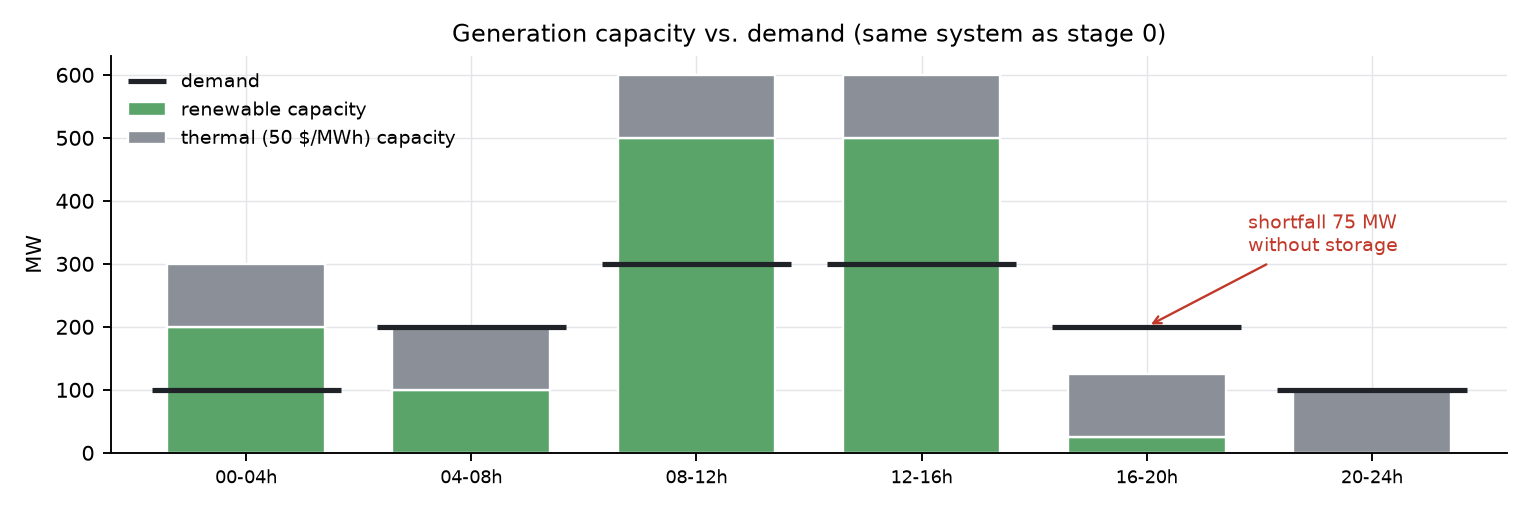
\includegraphics[width=0.8\textwidth]{figures/stage1/s1_system.png}
\end{center}

\textbf{Batteries.} The 800\,MWh battery of stage 0 is split into two batteries of 400\,MWh each. They are
identical except for their terminal value $w$:
\begin{center}\small
\begin{tabular}{@{}lcccccccc@{}}
\toprule
& $\bar s$ (MWh) & $s_0$ & $\alpha$ & $\beta$ & $\gamma$ & $\varepsilon=\zeta$ (\$/MWh) & $\bar p=\bar g$ (MW) & $w$ (\$/MWh)\\
\midrule
\textcolor{essA}{\textbf{A}} & 400 & 0 & 0.9 & 1 & 1 & 1 & 1\,000 & \textbf{40}\\
\textcolor{essB}{\textbf{B}} & 400 & 0 & 0.9 & 1 & 1 & 1 & 1\,000 & \textbf{55}\\
\bottomrule
\end{tabular}
\end{center}
Why this split:
\begin{itemize}
  \item \textbf{Comparable with stage 0.} Total storage stays 800\,MWh and every other parameter is
    Baldick's, so any difference from stage 0 comes from having two owners, not from a different system.
  \item \textbf{The two batteries differ only in $w$,} so the terminal value, and therefore its error, has a
    clear role. In this system the decisive number is \textbf{49\,\$/MWh}: selling a stored MWh at the
    price of 50 earns $50-\zeta=49$, and the morning round trip buys at 43.1 and needs $(43.1+\varepsilon)/
    \alpha=49$ to break even. A battery with $w<49$ sells its energy before the end of the day; with
    $w>49$ it keeps it. $w_A=40$ lies 9 below this threshold, $w_B=55$ lies 6 above it.
\end{itemize}
Code: \code{cases.stage1\_case(smax\_each=400, w=(40, 55))}; both numbers are arguments, so other splits
are one call away.

% =====================================================================
\section{Baldick's result on the new case}
% =====================================================================
\begin{center}
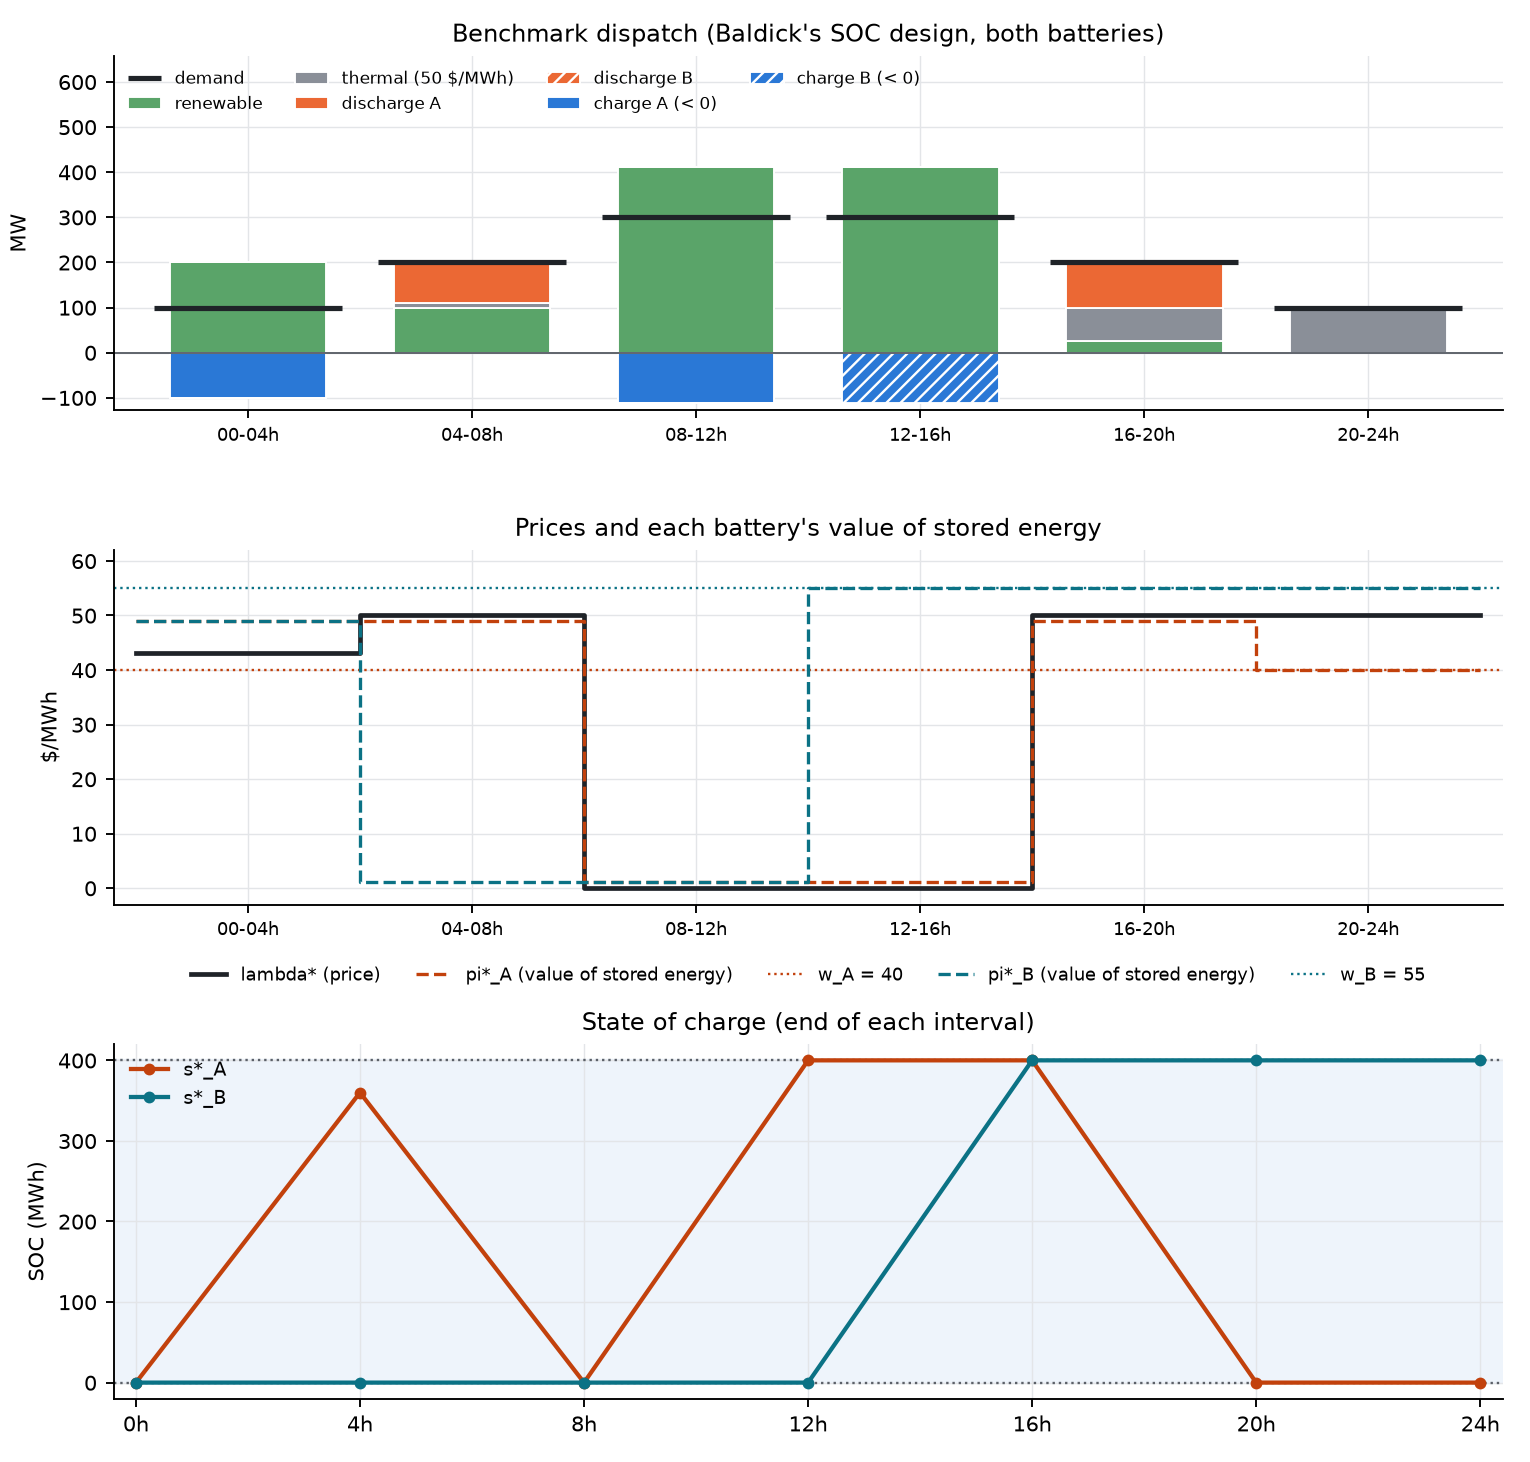
\includegraphics[width=0.86\textwidth]{figures/stage1/s1_benchmark.png}
\end{center}

\begin{center}\small
\begin{tabular}{@{}lrrrrrr@{}}
\toprule
Interval & 00--04h & 04--08h & 08--12h & 12--16h & 16--20h & 20--24h\\
\midrule
Demand (MW) & 100 & 200 & 300 & 300 & 200 & 100\\
Renewable used / available (MW) & 200 / 200 & 100 / 100 & 411 / 500 & 411 / 500 & 25 / 25 & 0 / 0\\
Thermal at 50 (MW) & 0 & 10 & 0 & 0 & 75 & 100\\
\midrule
\textcolor{essA}{A} charge / discharge (MW) & 100 / -- & -- / 90 & 111 / -- & -- & -- / 100 & --\\
\textcolor{essA}{A} SOC at end (MWh) & 360 & 0 & 400 & 400 & 0 & 0\\
\textcolor{essB}{B} charge / discharge (MW) & -- & -- & -- & 111 / -- & -- & --\\
\textcolor{essB}{B} SOC at end (MWh) & 0 & 0 & 0 & 400 & 400 & 400\\
\midrule
$\lamstar$ (\$/MWh) & 43.1 & 50 & 0 & 0 & 50 & 50\\
$\pi^\star_A$ (\$/MWh) & 49 & 49 & 1.11 & 1.11 & 49 & 40\\
$\pi^\star_B$ (\$/MWh) & 49 & 1.11 & 1.11 & 55 & 55 & 55\\
\bottomrule
\end{tabular}

\vspace{4pt}
\begin{tabular}{@{}lrr@{}}
\toprule
& Stage 1 (A + B) & Stage 0 (one battery)\\
\midrule
$SW^\star$ (\$) & $-17\,048.89$ & $-19\,448.89$\\
$SW_{\text{noESS}}$ (\$) & $-360\,000.00$ & $-360\,000.00$\\
$V=SW^\star-SW_{\text{noESS}}$ (\$) & $342\,951.11$ & $340\,551.11$\\
\bottomrule
\end{tabular}
\end{center}

How to read it:
\begin{itemize}
  \item \textbf{A is the trader.} It runs the morning round trip (buy 100\,MW at 43.1, sell 90\,MW at 50,
    exactly break-even), fills up on free renewable energy at 08--12h and empties at 16--20h, where its 100\,MW cover
    the 75\,MW shortfall and replace 25\,MW of thermal. Its value of stored energy $\pi^\star_A$ is 49 while it holds
    energy for a 50 sale, about 1 while energy is free, and $w_A=40$ in the last interval.
  \item \textbf{B is the store.} It fills on free energy at 12--16h and keeps all 400\,MWh to the end of the
    day, because each MWh is worth $w_B=55$ to it, more than the 49 a sale would earn. $\pi^\star_B=55$ from
    the moment it is full.
  \item \textbf{The prices are the stage-0 prices.} $\lamstar=(43.1,\,50,\,0,\,0,\,50,\,50)$ is unchanged.
  \item \textbf{$SW^\star$ is 2\,400\,\$ higher than in stage 0,} which is exactly $400\text{ MWh}\times
    (55-49)$. With one battery at $w=40$, those 400\,MWh were sold at 16--24h for a net 49; here B keeps them
    at 55. $V$ rises by the same amount.
  \item \textbf{Which battery does what is not unique.} Both are free to buy at 08--12h or 12--16h, and A
    could charge B's interval and vice versa: Baldick's LP returns one of several equally good splits. The
    welfare and the prices do not depend on that choice.
\end{itemize}
The equivalence still holds with two batteries: bids built from Baldick's own duals and quantities
(\code{B\_star}, both batteries) give $\Delta SW=0$ to floating-point precision.

% =====================================================================
\section{The two errors}
% =====================================================================
\subsection{Price error: the stage-0 model, now with a shared part}
Each owner gets its own forecast,
\[
\lamhat_{e,t}=\max\!\big(0,\;\lamstar_t+\sigma z_{e,t}\big),\qquad
z_{e,t}=\sqrt{\omega}\,\chi_t+\sqrt{1-\omega}\,\eta_{e,t},
\]
with $\chi$ common to both owners and $\eta_e$ owner-specific (AR(1), unit variance). With one battery $\omega$
had no effect; with two it sets how alike the owners' forecasts are: $\omega=0$ independent forecasts,
$\omega=1$ the same forecast (both buy the same data). The errors of both owners are drawn together, once per
draw, so $\chi$ is truly shared.

\subsection{Terminal-value error (new)}
Each owner estimates what its stored energy will be worth at the end of the day:
\[
\boxed{\;\what_e=\max\!\big(0,\;w_e+\sigma_w\,z_{w,e}\big),\qquad z_{w,e}\sim N(0,1)\text{ iid}\;}
\]
one draw per battery and scenario, constant over the day, independent of the price error.
\begin{itemize}
  \item \textbf{Why an error on $w$.} $w$ is the owner's view of tomorrow: tomorrow's prices, its own
    commitments, its degradation outlook. It is as much a forecast as $\lamhat$, and Baldick's design asks the
    owner to submit it. In the current design it never reaches the ISO, but it shapes the bid: it is the
    end-point of the owner's self-schedule (M3) and fixes $\pi_T$.
  \item \textbf{Where it enters.} Only in the owner-built bids: \code{B\_fcst} uses $(\lamhat_e,\what_e)$,
    \code{B\_priv} uses $\what_e$. The benchmark and the welfare keep the true $w_e$, exactly as the price error
    leaves $\lamstar$ untouched.
  \item \textbf{Why it matters here.} Because of the 49\,\$/MWh threshold (\S3), a $\what_e$ on the wrong side
    of 49 flips the owner's end-of-day decision: an A with $\what_A>49$ keeps its energy instead of covering
    the 16--20h shortfall; a B with $\what_B<49$ sells energy it should have kept. At $\sigma_w=5$ the chance
    of crossing is $P(z>1.8)=3.6\%$ for A and $P(z<-1.2)=11.5\%$ for B.
  \item \textbf{Floor.} $\what_e\ge0$, the same floor as the price: stored energy can always be kept, so it
    is never worth less than nothing.
  \item \textbf{Seeds.} $z_{w,e}$ has its own stream, \code{RunSettings.seed\_w(d)}, so draw $d$ has the same
    $z_w$ whatever $\sigma$, $\omega$ or $\sigma_w$ are (common random numbers for both errors).
\end{itemize}

One draw ($d=0$, $\sigma=5$, $\omega=0.5$, $\sigma_w=5$): the error shapes, the two forecasts, and the two
terminal-value estimates ($\what_A=38.2$, $\what_B=52.8$, both on the correct side of 49).
\begin{center}
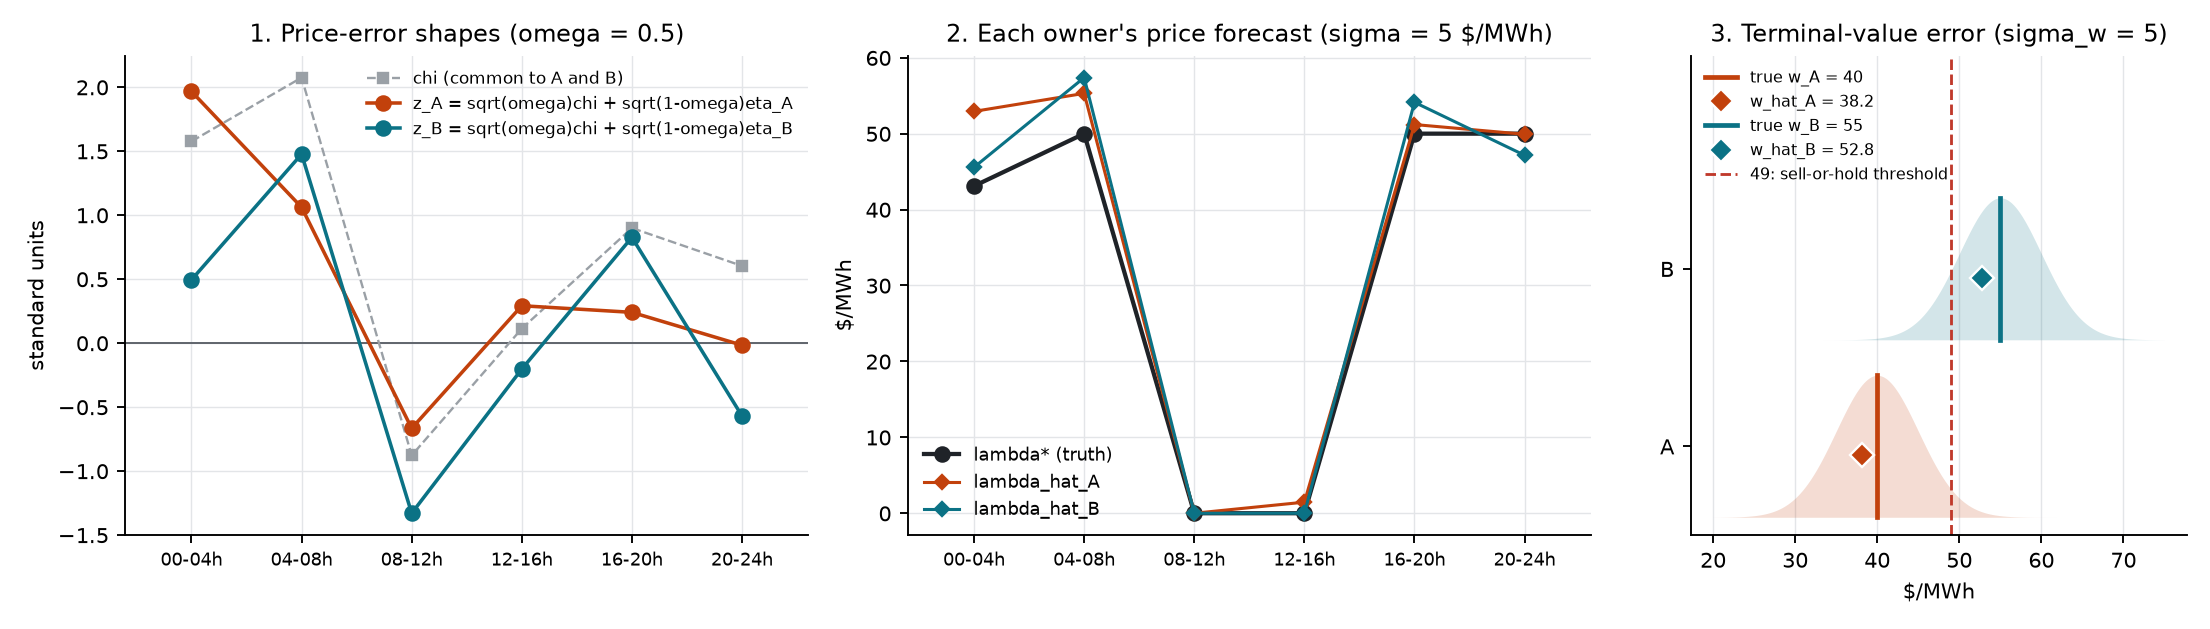
\includegraphics[width=\textwidth]{figures/stage1/s1_errors.png}
\end{center}

% =====================================================================
\section{First check at zero error: the two bids cross}
\label{sec:cross}
% =====================================================================
Before any error, each owner builds its bid from its own self-schedule at the \emph{true} prices
(\code{B\_star\_p}). With one battery this cost 1.30\% of $V$. With two it costs \textbf{38.1\%}, sheds
124\,MWh at 20--24h, and leaves 6\,976\,MWh of the day-ahead schedule undeliverable.
\begin{center}
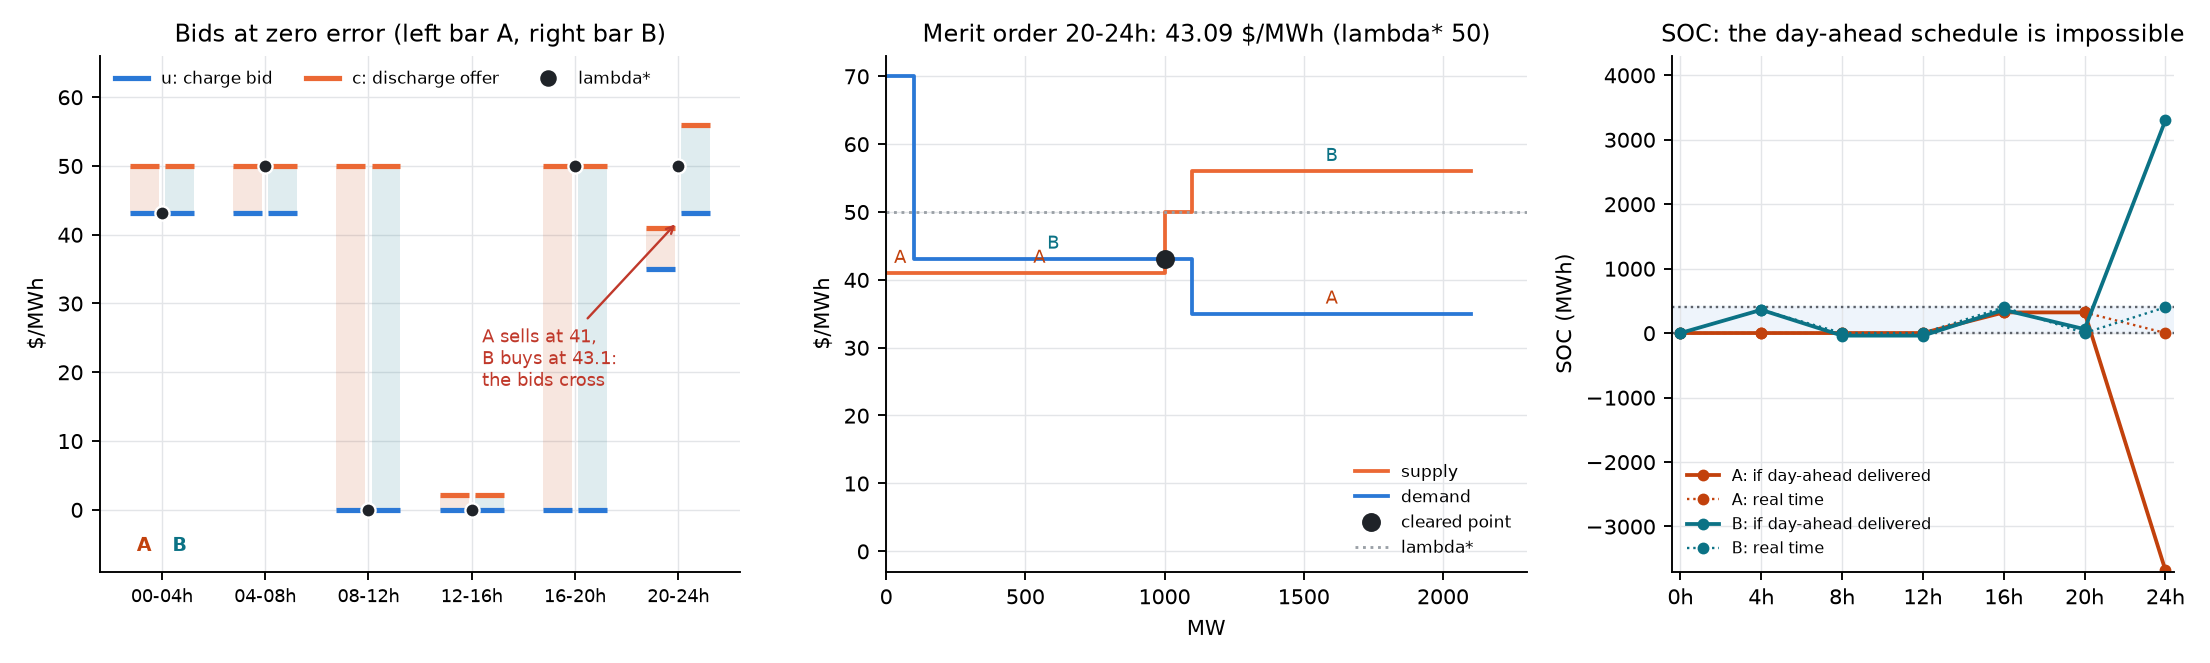
\includegraphics[width=\textwidth]{figures/stage1/s1_zero_error.png}
\end{center}
\textbf{Mechanism.} The quantity rule sends two blocks per side: the planned quantity at $u+\delta$ (charge) or
$c-\delta$ (discharge), and \emph{all remaining power}, $\bar p-p^\circ$ or $\bar g-g^\circ$, at $u-\delta$ or
$c+\delta$. With Baldick's non-binding power limits of 1\,000\,MW, this second block is up to 1\,000\,MW
regardless of how much energy the battery holds. At 20--24h A offers to sell at $c_A=41$ ($\pi_A=w_A=40$
plus $\zeta$) and B bids to buy at $u_B=43.1$. The bids cross, so the market clears A selling 1\,000\,MW
and B buying 900\,MW at 43.09\,\$/MWh: the two batteries trade with each other. Neither can deliver (A is
almost empty, B almost full). With one battery this cannot happen, because a battery cannot trade with
itself.

In real time each battery does what its SOC allows: A delivers 80\,MW, B still charges 111\,MW, and the
system sheds 31\,MW to serve that charge (below). The real-time rule treats a battery's feasible charge as
firm load, even when that means shedding; with one battery that never occurred.
\begin{center}
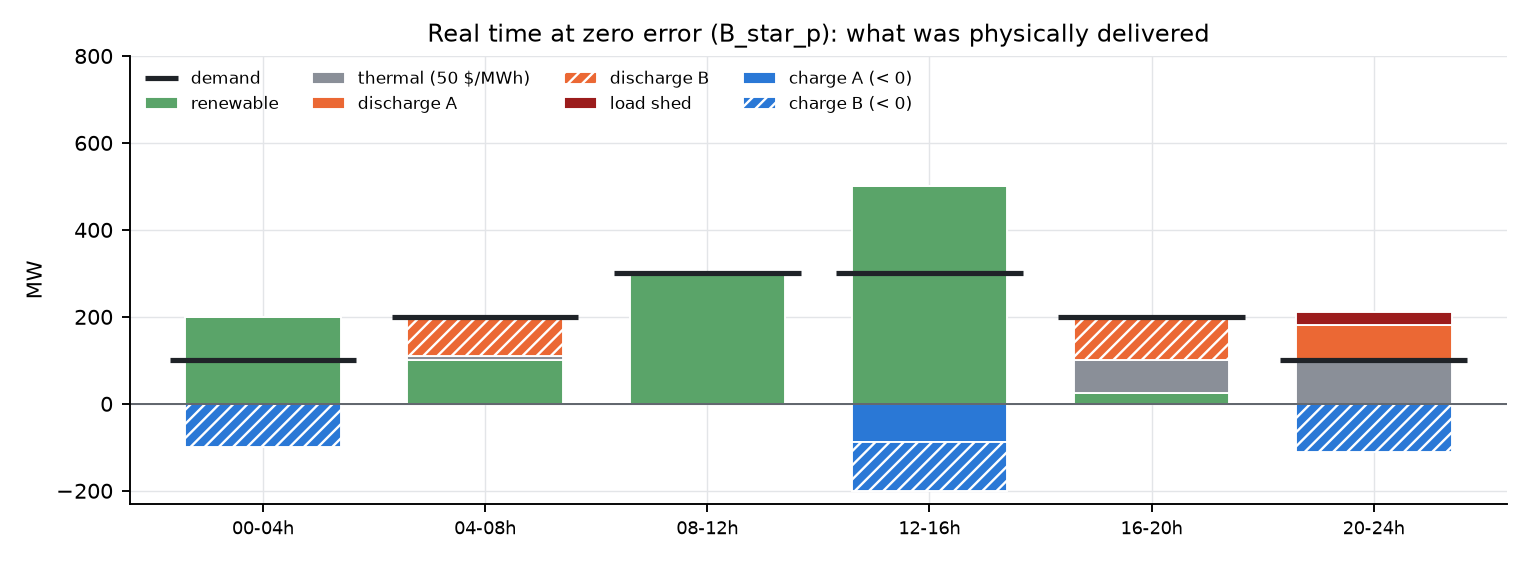
\includegraphics[width=0.8\textwidth]{figures/stage1/s1_zero_error_rt.png}
\end{center}

\textbf{This dominates every error result.} A first exploratory run (40 draws, $\omega=0.5$, current rule)
gives mean losses of 21--102\% of $V$ with load shed in 52--100\% of draws, and no clear pattern in
$\sigma$ or $\sigma_w$: the crossing, not the errors, decides the outcome. The same zero-error check under
alternatives (30 draws for the error column):
\begin{center}\small
\begin{tabular}{@{}lccc@{}}
\toprule
Quantity rule / case & \code{B\_star\_p} loss & $\sigma=0$, $\sigma_w=5$: mean loss & draws shedding\\
\midrule
Current: 2nd block = all remaining power & 38.1\% & 22.4\% & 57\%\\
Plan only (no 2nd block) & 84.6\% & 84.6\% & 100\%\\
2nd block capped by the battery's own SOC plan & \textbf{2.0\%} & \textbf{2.0\%} & \textbf{0\%}\\
Current rule, $\bar p=\bar g=100$\,MW & 0.6\% & 0.7\% & 0\%\\
\bottomrule
\end{tabular}
\end{center}
``Capped by the SOC plan'': the second block offers only what the battery could still absorb or deliver from
the SOC its own plan reaches, $\min\!\big(\bar p,(\bar s-\gamma s^\circ_{t-1})/(\alpha\Delta T)\big)-p^\circ_t$ on
the charge side and $\min\!\big(\bar g,(\gamma s^\circ_{t-1}-\underline s)/(\beta\Delta T)\big)-g^\circ_t$ on
the discharge side. Removing the second block altogether is worse, because those blocks are also what lets the
market move energy from one battery to the other when their plans overlap (both plan to buy the same free
energy).

\begin{center}
\fcolorbox{warn}{warn!6}{\begin{minipage}{0.93\textwidth}\small
\textbf{Decisions needed before the notebook.}
\begin{enumerate}
  \item \textbf{Quantity rule.} Keep the current rule (and report the crossing as a finding of the current
    design with independent owners), cap the second block by the SOC plan (recommended: a battery should not
    offer energy it cannot have), or change the case to realistic power limits. This is the bid-curve topic
    that was already next in the plan.
  \item \textbf{Real-time priority.} Should real time curtail a battery's charge before it sheds load? With
    one battery this never mattered; with two it does.
\end{enumerate}
\end{minipage}}
\end{center}

% =====================================================================
\section{Proposed settings and the notebook}
% =====================================================================
\textbf{Settings} (one CSV per setting in \code{results/stage1/}, 150 draws each, base seed 42, common random
numbers):
\begin{center}\small
\begin{tabularx}{\textwidth}{@{}llX@{}}
\toprule
Parameter & Values & Why\\
\midrule
$\sigma$ (\$/MWh) & 0, 1, 2, 5, 10, 20 & same as stage 0, so the curves can be laid on top of each other\\
$\sigma_w$ (\$/MWh) & 0, 2, 5, 10 & from ``never crosses 49'' to ``often crosses'' for both batteries\\
$\omega$ & 0, 0.5, 1 & independent, partly shared, identical forecasts\\
$\rho$, bias, $\psi$, rule & 0, 0, 10, \code{prelimit} & as in stage 0\\
Deterministic & \code{B\_star}, \code{B\_star\_p}, \code{B\_priv} ($\psi=0,10,50$) & gate and references\\
\bottomrule
\end{tabularx}
\end{center}
$6\times4\times3=72$ stochastic settings, 10\,800 draws, about 20 minutes.

\textbf{Notebook \code{notebooks/stage\_1.ipynb}}, same format as stage 0: (1) the system and the two
batteries, (2) Baldick's benchmark, figure and table, (3) the two errors on one draw, (4) the bids of A and B,
(5) day-ahead clearing with both bids, (6) real time, (7) one draw end to end with an explorer, (8)
deterministic gate (\code{B\_star} $\Delta SW=0$ with two batteries; $\sigma=\sigma_w=0$ reproduces
\code{B\_star\_p}), (9) results: loss over $(\sigma,\sigma_w)$ as a heatmap, the effect of $\omega$, paired
comparisons, (10) no simultaneous charge and discharge, (11) summary.

% =====================================================================
\section{Code added for stage 1}
% =====================================================================
\begin{itemize}
  \item \code{cases.stage1\_case(smax\_each, w)}: the system above.
  \item \code{ErrorModel.sigma\_w} and \code{forecasts.terminal\_values}: the terminal-value error.
  \item \code{RunSettings.seed\_w(d)}: its own seed stream.
  \item \code{runner.run\_draw}: draws all owners' price forecasts together (so $\chi$ is shared), draws
    $\what$, builds \code{B\_fcst} and \code{B\_priv} with it; rows gain \code{sigma\_w} and \code{w\_hat\_e}.
  \item \code{scripts/make\_stage1\_figures.py}: every figure and number in this document.
\end{itemize}
Stage 0 is unaffected: rerunning all 1\,506 stage-0 draws reproduces \code{results/stage0/} to $10^{-12}$, and
all 21 tests pass (two new: the two-battery gate and the $\what$ error).

\end{document}
